\documentclass[11pt]{article}

\usepackage[margin=1in]{geometry}
\usepackage{amsmath, amssymb, amsfonts}
\usepackage{microtype}
\usepackage{parskip}
\usepackage{tikz}
\usetikzlibrary{positioning, arrows.meta, fit, backgrounds}
\usepackage{hyperref}

\newcommand{\E}{\mathbb{E}}
\newcommand{\one}{\mathbf{1}}
\newcommand{\pzero}{\pi_{0}}
\newcommand{\pprime}{\pi'}
\newcommand{\sloss}[2]{\bigl(#1 - #2\bigr)_{+}}
\newcommand{\that}{\hat t}
\newcommand{\CVaR}{\mathrm{CVaR}}

\title{From the Mean Audit to the CVaR Audit\\\large A Narrative on Two Versions of the Same Idea}
\author{}
\date{}

\begin{document}
\maketitle

\section*{The data we have, and the data we wish we had}

We deployed a policy $\pzero$, the \emph{logger}, and we collected its responses along with two scores per response. The cheap one is a judge score $S$, produced by a smaller model. The expensive one is an oracle label $Y$, produced by a careful human or a much stronger model. Because the oracle is expensive, we only have it on a slice of the data, but on that slice we have both $S$ and $Y$, and that is what makes everything that follows possible.

What we actually want is the value of a different policy, $\pprime$, the \emph{target}. We have responses from $\pprime$ too, but only their judge scores: no oracle labels. So the question is whether the judge score is enough to estimate what we would have computed if we had paid for oracle labels under $\pprime$.

The whole framework rests on one bridge: a function $f$ trained on the logger's oracle slice that turns a judge score into a prediction of the oracle label, $f(S) \approx \E[Y \mid S]$. If that bridge holds when we cross over to $\pprime$, we can take the average of $f(S)$ over fresh draws under $\pprime$ and call it an estimate of $\E_{\pprime}[Y]$. The audit's job is to check whether the bridge holds.

\section*{The mean audit, in one sentence}

The main paper's audit is a one-sample $t$-test on a single residual.

For each row $i$ in an audit slice drawn under $\pprime$ --- a slice on which we deliberately spent oracle budget so that we have both $S_i$ and $Y_i$ --- compute
\[
r_i \;=\; Y_i - f(S_i).
\]
This is the gap between the calibrator's prediction and the truth, on data the calibrator never saw. If the bridge holds, the gap should average to zero across the audit slice. If the calibrator was trained on a logger that answers more verbosely than $\pprime$, or that scores higher on prompts that $\pprime$ never sees, the gap will not average to zero, and that is exactly the failure we want to catch.

The test statistic is the obvious one,
\[
T \;=\; \frac{\bar r}{\mathrm{SE}(\bar r)},
\]
where $\bar r$ is the audit-slice mean of $r_i$ and the standard error has two pieces. The first is the usual sample-variance term $\widehat{\mathrm{Var}}(r_i)/n_a$. The second is the part most analyses forget: the calibrator $f$ is itself estimated from a finite oracle slice, so $f$ has its own noise, and $r_i$ inherits some of it. The paper handles this by refitting the calibrator with each oracle fold held out --- a jackknife on the calibrator's training data --- and propagating that variance into $\mathrm{SE}(\bar r)$. The paper calls this the OUA jackknife, where OUA stands for ``oracle uncertainty aware.''

\begin{figure}[h]
\centering
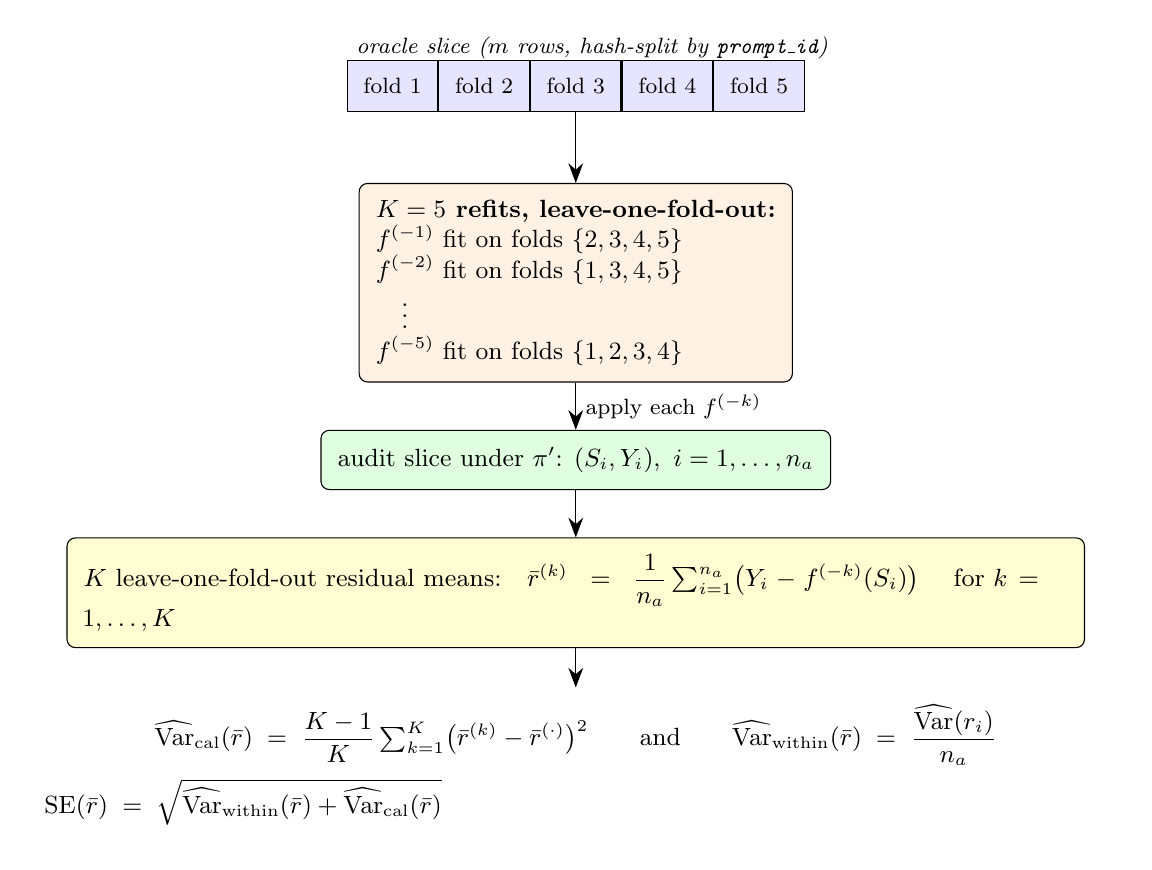
\begin{tikzpicture}[
  >={Stealth[length=2.5mm]},
  font=\small,
  fold/.style={draw, minimum width=1.15cm, minimum height=0.65cm, fill=blue!10, font=\footnotesize},
  box/.style={draw, rounded corners=3pt, inner sep=6pt, align=left},
  node distance=0.55cm and 0.6cm
]
  % Oracle slice header
  \node[font=\itshape\footnotesize] (header) {oracle slice ($m$ rows, hash-split by \texttt{prompt\_id})};

  % 5 fold cells in a row, abutting
  \node[fold, below=0.15cm of header.west, anchor=north west] (f1) {fold 1};
  \node[fold, right=0pt of f1] (f2) {fold 2};
  \node[fold, right=0pt of f2] (f3) {fold 3};
  \node[fold, right=0pt of f3] (f4) {fold 4};
  \node[fold, right=0pt of f4] (f5) {fold 5};

  % Refits box
  \node[box, fill=orange!10, below=0.9cm of f3] (refits) {%
    \textbf{$K=5$ refits, leave-one-fold-out:}\\
    $f^{(-1)}$ fit on folds $\{2,3,4,5\}$\\
    $f^{(-2)}$ fit on folds $\{1,3,4,5\}$\\
    \quad $\vdots$\\
    $f^{(-5)}$ fit on folds $\{1,2,3,4\}$};
  \draw[->] (f3.south) -- (refits.north);

  % Audit slice
  \node[box, fill=green!12, below=0.6cm of refits] (audit) {%
    audit slice under $\pprime$: $(S_i, Y_i),\ i = 1, \dots, n_a$};
  \draw[->] (refits.south) -- (audit.north) node[midway, right, font=\footnotesize] {apply each $f^{(-k)}$};

  % K residual means
  \node[box, fill=yellow!18, below=0.6cm of audit, text width=12.5cm] (means) {%
    $K$ leave-one-fold-out residual means:\quad $\bar r^{(k)} \;=\; \dfrac{1}{n_a}\sum_{i=1}^{n_a} \bigl(Y_i - f^{(-k)}(S_i)\bigr)$ \quad for $k = 1,\dots,K$};
  \draw[->] (audit.south) -- (means.north);

  % Variance / SE
  \node[box, draw=none, below=0.5cm of means, text width=13.5cm] (var) {%
    \centering
    $\widehat{\mathrm{Var}}_{\mathrm{cal}}(\bar r) \;=\; \dfrac{K-1}{K}\sum_{k=1}^{K} \bigl(\bar r^{(k)} - \bar r^{(\cdot)}\bigr)^{2}
    \qquad\text{and}\qquad
    \widehat{\mathrm{Var}}_{\mathrm{within}}(\bar r) \;=\; \dfrac{\widehat{\mathrm{Var}}(r_i)}{n_a}$\\[4pt]
    $\mathrm{SE}(\bar r) \;=\; \sqrt{\widehat{\mathrm{Var}}_{\mathrm{within}}(\bar r) + \widehat{\mathrm{Var}}_{\mathrm{cal}}(\bar r)}$};
  \draw[->] (means.south) -- (var.north);
\end{tikzpicture}
\caption{The OUA (oracle-uncertainty-aware) jackknife. The oracle slice is split into $K$ folds. The calibrator is refit $K$ times, each time leaving one fold out, and applied to the audit slice. The variability across the $K$ leave-one-fold-out residual means $\bar r^{(k)}$ supplies the calibration component of the standard error; the usual within-audit-slice term supplies the rest.}
\label{fig:oua}
\end{figure}

Reject when $|T| > 1.96$. The hypothesis being tested has a name in the paper: \textbf{(T1)}, the mean transport condition, $\E_{\pprime}[Y - f(S)] = 0$. The action on rejection is also fixed: flag the surrogate-only level estimate as biased for $\pprime$, optionally report the size and sign of $\bar r$ as an estimate of the bias, and either recalibrate using policy-specific oracle data or refuse the level claim and fall back to oracle-only inference. Crucially, even when an absolute level fails, the relative ranking across policies that all pass the audit can still be valid; the paper is explicit about that distinction.

That is the whole story of the mean audit. One residual per row, average it, divide by a careful standard error, compare to a normal cutoff, decide.

\section*{What changes when we move to the tail}

The CVaR estimand is the average of the worst $\alpha$-fraction of responses --- at the headline $\alpha = 0.10$, the worst tenth. Two things change relative to the mean.

First, the estimator is no longer ``apply $f$ and average.'' To compute a CVaR you need a threshold $\that$ that locates the tail, and then you need to know, for the responses below that threshold, how far below they typically fall. The variational identity used throughout the appendix says these two pieces can be optimised jointly: the CVaR equals the maximum over candidate thresholds $t$ of $t - \alpha^{-1} \E_{\pprime}\!\left[\sloss{t}{Y}\right]$, where $\sloss{t}{Y} = \max(t - Y, 0)$ is the shortfall below $t$. The maximiser is the true $\alpha$-quantile, and the maximum is the CVaR. So the algorithm is to fit a \emph{shortfall calibrator} $g_t(S) \approx \E\!\left[\sloss{t}{Y} \mid S\right]$ for each $t$ on a grid, average it over fresh draws under $\pprime$ to get $\bar Z_t$, and pick the $t$ that maximises $t - \bar Z_t / \alpha$. Call that maximiser $\that$.

Second, the audit now has two ways to fail. The mean audit could only fail one way: the calibrator might not transfer in mean. The CVaR audit can fail that way too, but it can also fail because $\that$ landed in the wrong place. If $\that$ is below the true quantile we are evaluating the CVaR at the wrong horizon; if it is above we are doing the same. Either way the level estimate is wrong, and the audit needs to notice.

So the appendix uses two moments per row, not one.

\section*{The first new moment: did $\that$ land at the right quantile?}

By definition, the $\alpha$-quantile of $Y$ has exactly an $\alpha$-fraction of mass at or below it. So if $\that$ is the right place, the indicator
\[
g_{1,i} \;=\; \one\{Y_i \le \that\} - \alpha
\]
should average to zero on the audit slice. This is a quantile check in indicator form: the share of audit observations below $\that$ minus the level we wanted. A positive average means $\that$ is too high (too many rows below it); a negative average means $\that$ is too low. The strict mathematical statement requires a small caveat we return to below: if $Y$ has a point mass at the true quantile, this moment can be nonzero even at a valid threshold, and the appendix flags that explicitly with a no-atom assumption.

\section*{The second new moment: does the shortfall calibrator transfer?}

The same logic that gave us the mean residual gives us a shortfall residual, but at the threshold the algorithm chose:
\[
g_{2,i} \;=\; \sloss{\that}{Y_i} - g_{\that}(S_i).
\]
This is the gap between the actual shortfall of $Y_i$ below $\that$ and the calibrator's prediction of that shortfall. If the calibrator transfers from logger to target at the threshold $\that$, the gap averages to zero. If it does not --- if, say, the shape of the lower tail looks different under $\pprime$ than the calibrator learned on $\pzero$ --- the gap moves and the audit catches it.

This is the threshold-indexed analogue of the main paper's mean residual. The transport condition it is testing is no longer the mean version $(T1)$ but a stronger, $t$-indexed version: $\E_{\pprime}\!\left[\sloss{t}{Y} \mid S\right] = \E_{\pzero}\!\left[\sloss{t}{Y} \mid S\right]$ for $t$ in a neighbourhood of $\that$. We added a new footnote to the appendix stating exactly this.

\section*{Combining the two moments}

We now have a two-vector of audit residuals,
\[
\bar g \;=\; \begin{pmatrix} \overline{g_{1}} \\ \overline{g_{2}} \end{pmatrix},
\]
and the natural test is the Wald quadratic form
\[
W_n \;=\; \bar g^{\top}\, \hat\Sigma^{-1}\, \bar g,
\]
which compares to a chi-squared distribution with two degrees of freedom. Reject when $W_n > 5.99$. The covariance $\hat\Sigma$ is estimated by a paired bootstrap that resamples prompt clusters --- and crucially re-runs the threshold maximisation inside each replicate, because $\that$ is itself a noisy quantity and pretending it is fixed would make the variance estimate too small.

The two moments are designed to fail in distinct ways. Holding the calibrator fixed and shifting $\that$ moves $g_1$ but leaves $g_2$ at zero in expectation. Adding a constant offset to the calibrator moves $g_2$ but leaves $g_1$ at zero, because the variational maximum is invariant to additive shifts in the calibrator. The appendix verifies this experimentally: in a Monte Carlo study where one moment is perturbed at a time, only the corresponding moment moves.

\section*{Why the mean audit is just the CVaR audit at $\alpha = 1$}

This is the clean way to remember the relationship. Take $\alpha = 1$ and assume $Y \in [0,1]$. Then:

\begin{itemize}
\item $g_{1,i} = \one\{Y_i \le \that\} - 1$. But $\that$ at $\alpha=1$ is the maximum of $Y$, so the indicator is identically $1$ and $g_{1,i} \equiv 0$. The threshold check becomes vacuous because there is no tail to localise.
\item $g_{2,i} = (\that - Y_i)_+ - g_{\that}(S_i)$. With $\that = 1$ and $Y_i \in [0,1]$, $(\that - Y_i)_+ = 1 - Y_i$, and $g_{\that}(S_i)$ converges to $1 - f(S_i)$. So $g_{2,i} \to (1 - Y_i) - (1 - f(S_i)) = f(S_i) - Y_i = -r_i$.
\item $W_n$ collapses to a scalar quadratic in $\bar r$, which is just $T^2$ in the standard normal limit.
\end{itemize}

So the CVaR audit is the threshold-indexed generalisation of the mean audit. The mean audit lives at $\alpha = 1$ where the tail is the whole distribution and the threshold check is trivial; as $\alpha$ shrinks the threshold check becomes a real constraint and the shortfall residual replaces the mean residual.

\section*{What can still go wrong, and what we assume to stop it}

The appendix is honest about the regularity its $\chi^{2}_{2}$ claim depends on, especially after the recent footnote pass. Four assumptions matter.

\textbf{No atom at the quantile.} If $\Pr_{\pprime}(Y = q_{\alpha}(\pprime)) > 0$, then $g_1$ does not have mean zero even at the correct threshold, because the indicator $\one\{Y \le q_\alpha\}$ jumps by the size of the atom and the share at or below the quantile is not exactly $\alpha$. This is a real issue if $Y$ comes from a discrete or rounded grading scheme. The cleanest fix is to assume continuity at $q_\alpha$, which is what the appendix now does explicitly. If continuity is implausible, the alternatives are randomised tie handling or an inequality-based audit, both of which complicate the test.

\textbf{Shortfall transport, not just mean transport.} The mean transport condition $(T1)$ is enough for the main paper because the estimand only involves means. The CVaR estimand involves shortfalls, and the relevant transport assumption is that the shortfall calibrator transfers across policies, not just the mean calibrator. This was implicit in earlier drafts and is now stated formally in a footnote at the $g_2$ paragraph.

\textbf{Unique interior maximiser.} The CVaR estimator is the value of a maximised objective. If the objective is flat at the top, $\that$ is not pinned down, and the asymptotic distribution of $W_n$ is no longer $\chi^{2}_{2}$ in any clean way. With a continuous tail this is generically fine; with discrete labels and a coarse grid it can bite. The appendix's response is to state this as a regularity condition rather than to prove it from primitives.

\textbf{A valid clustered bootstrap.} The variance $\hat\Sigma$ has to actually estimate the variance of $\bar g$. The paired-bootstrap-with-re-maximisation construction is what gives this; an alternative that fixes $\that$ would underestimate variance and produce too many rejections.

\section*{Decision logic, on both audits}

Both audits end the same way. A rejection is a signal, not a sentence. If the audit rejects, the right move is either to recalibrate using oracle data drawn under the offending policy --- which absorbs the failure into the calibrator and restores transport --- or to refuse the level claim for that policy and fall back to oracle-only inference. The latter is the conservative path the appendix takes for the unhelpful policy, where the audit rejects on $19$ of $20$ seeds: we report the rejection, we do not interpret the level estimate as calibrated, and we treat the rejection itself as the useful diagnostic.

What does \emph{not} happen, and what the appendix used to imply too strongly before the recent fix, is interpreting a rejected interval as evidence that the estimator was nevertheless on the right track. If the audit rejects, the level and its CI are not calibrated. The audit's job is detection.

\section*{The one-line summary}

The mean audit asks ``does $f$ predict $Y$ on average under $\pprime$?'' and uses one moment to answer. The CVaR audit asks the same question one level deeper --- ``does $g_t$ predict the shortfall, and is $\that$ in the right place?'' --- and uses two moments to answer. Everything else, including how variances are estimated, how the bootstrap clusters, and how rejections feed back into recalibrate-or-refuse, is the same machinery applied to a different estimand.

\end{document}
